\begin{abwframe}
\ABWTitle{Come join the PC-BAN/DSBA/BITM!}
\node[anchor=north west,inner sep=0pt] at (42bp,-133bp) {\begin{minipage}[t]{610bp}\setlength{\parskip}{9bp}\fontsize{20}{24}\selectfont
\textbullet\ The Programme Committee is a statutory body where students and lecturers discuss the quality of education.\par
\textbullet\ It advises on curriculum design, quality assurance and policy-making.\par
\textbullet\ At least six meetings each academic year, with equal student and lecturer representation.\par
\textbullet\ An honourable membership: represent your fellow students.\par
\textbullet\ A grant is available from the UvA Profiling Fund.\par
\end{minipage}};
\node[anchor=north west,inner sep=0pt] at (690bp,-126bp) {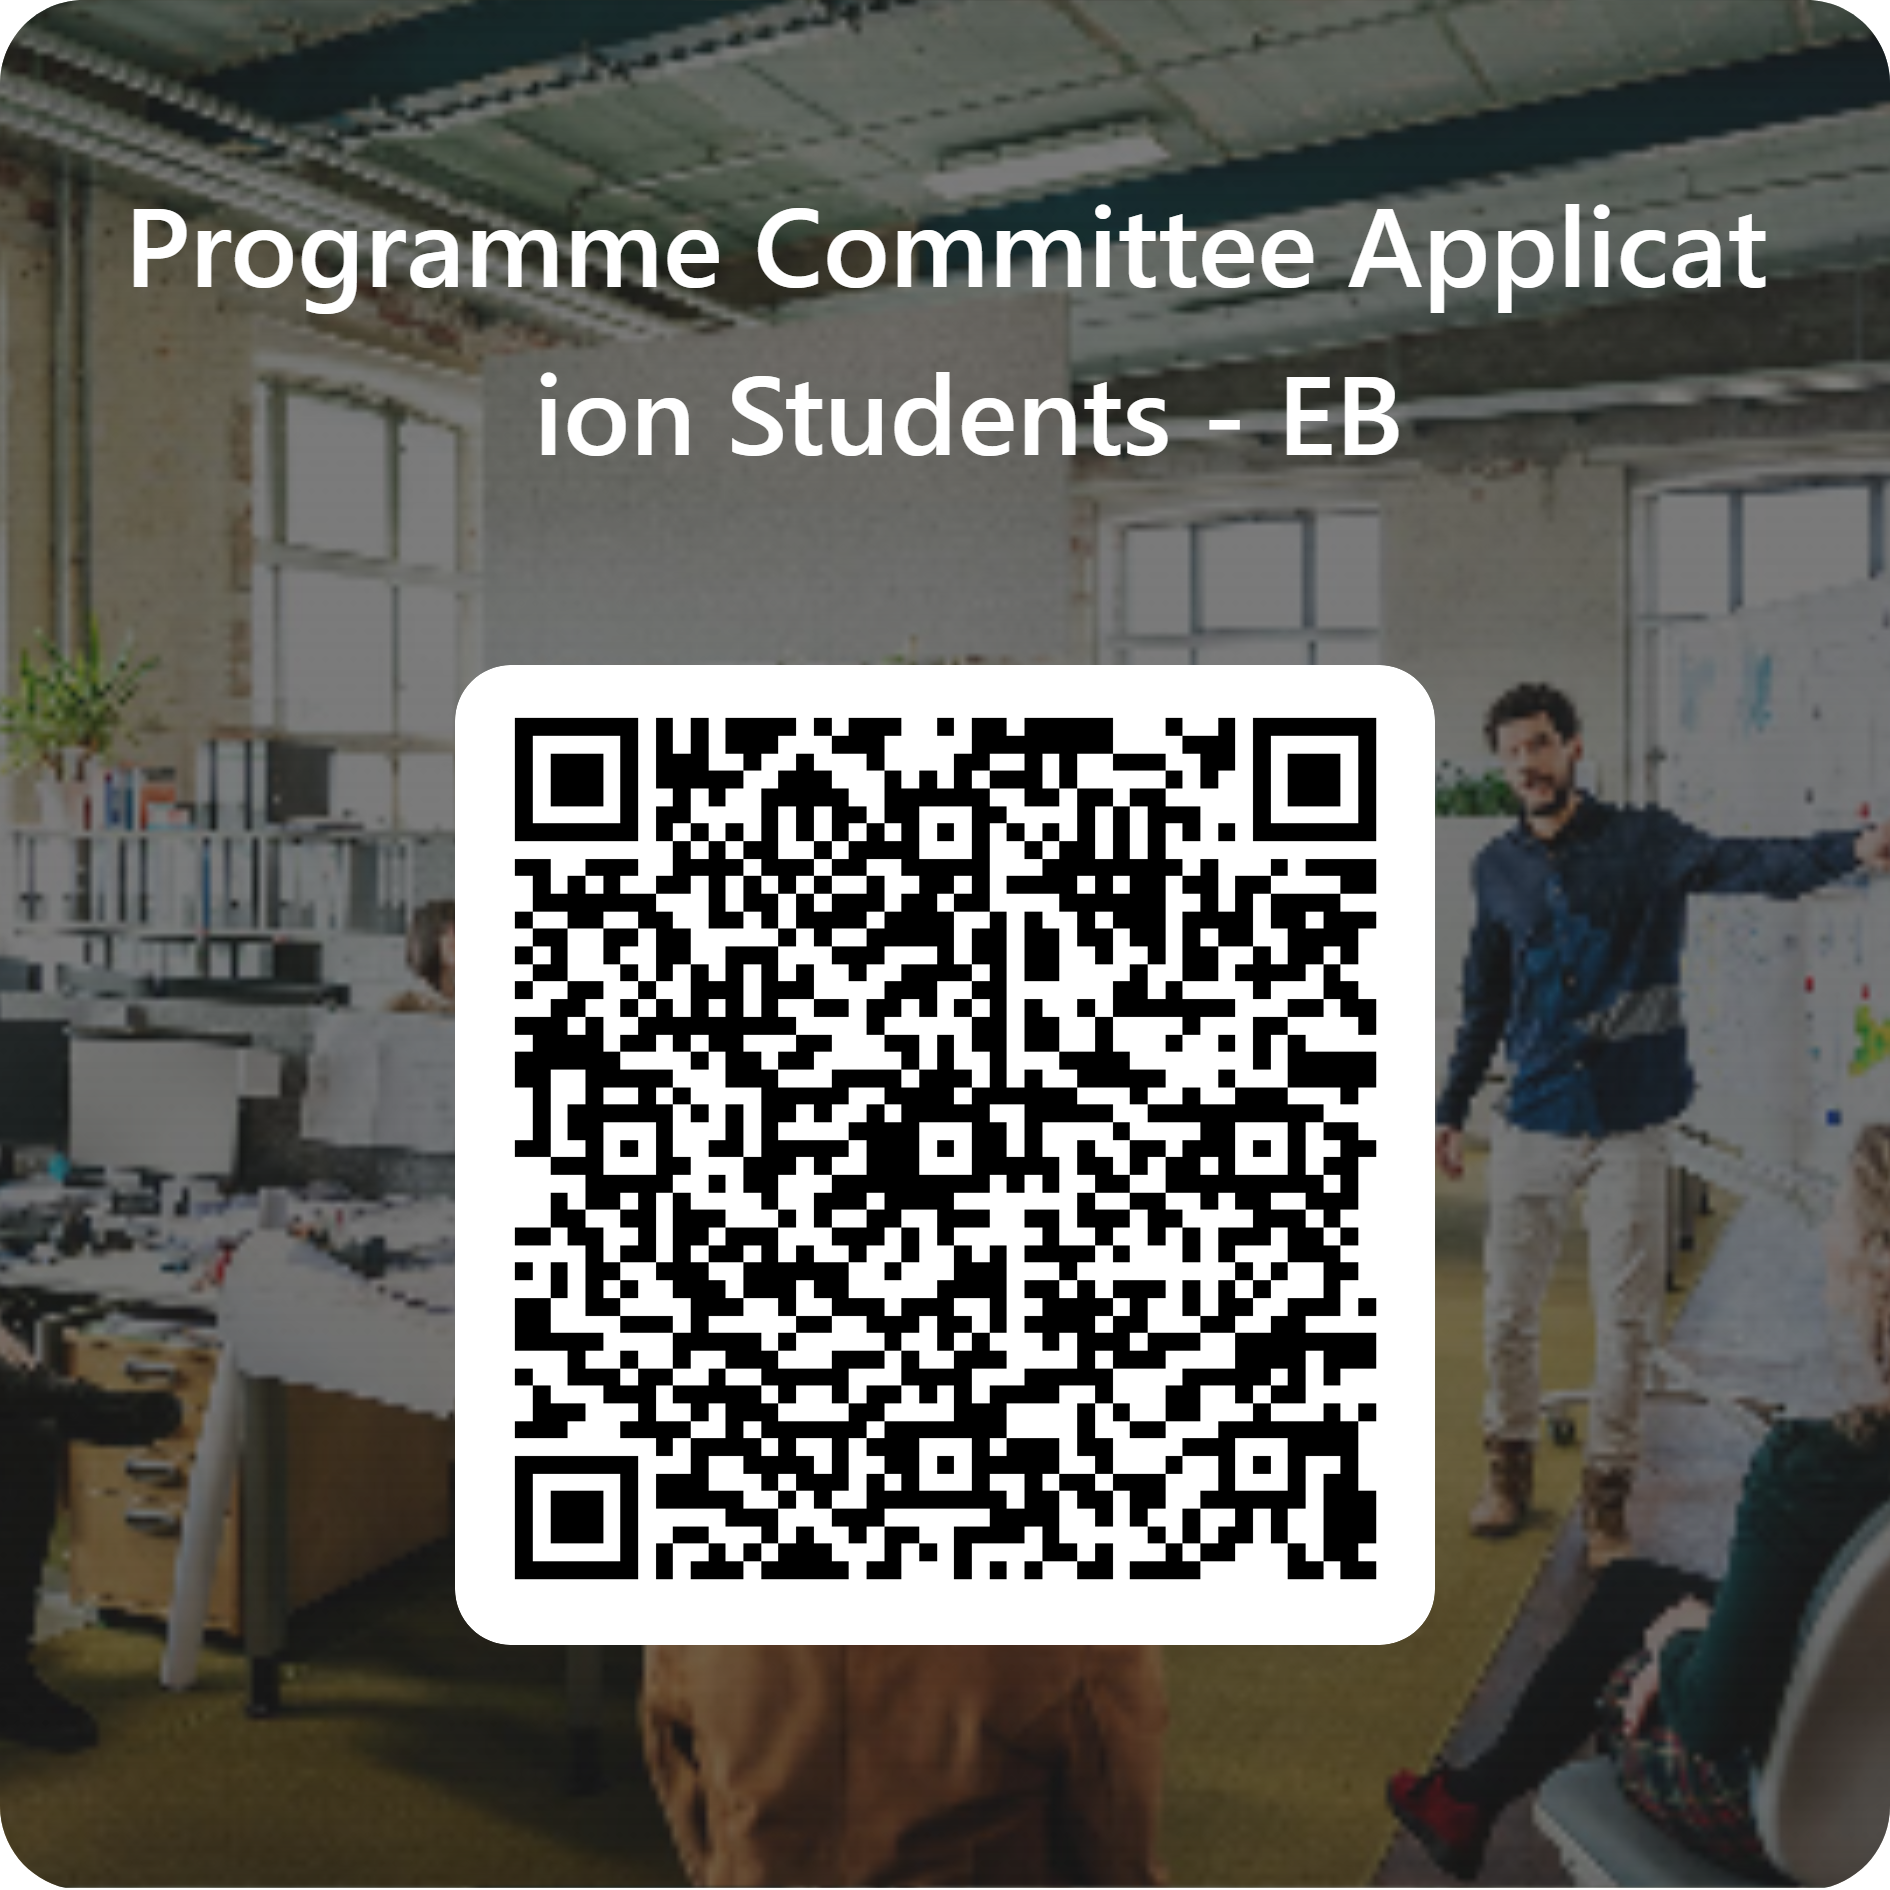
\includegraphics[width=210bp]{assets/programme-committee-2026/programme-committee-application-qr.png}};
\node[anchor=north] at (795bp,-400bp) {\begin{minipage}{220bp}\centering\color{cC00000}\bfseries\fontsize{16}{19}\selectfont Interested? Scan the QR code and complete the form.\end{minipage}};
\node[anchor=north] at (795bp,-468bp) {\begin{minipage}{220bp}\centering\color{c505150}\fontsize{14}{17}\selectfont Deadline: 13 September\end{minipage}};
\node[anchor=south west,inner sep=0pt] at (42bp,-478bp) {\color{c7F7F7F}\fontsize{8}{10}\selectfont Recruitment information and QR code: UvA Programme Committee recruitment 2026.};
\ABWFooter{\insertframenumber}
\end{abwframe}